% KAPITEL 2: Theoretische Grundlagen (02_theorieteil.tex)


\section{Theoretische Grundlagen und Stand der Technik}
\label{chap:theorie}

Das vorliegende Kapitel erarbeitet das theoretische Fundament dieser Arbeit und führt in die Problematik der Strommessung unter dem Einfluss magnetischer Störfelder ein. Zunächst erfolgt eine detaillierte Betrachtung von Messstromwandlern. Neben dem konstruktiven Aufbau und den verschiedenen Bauformen liegt ein besonderer Schwerpunkt auf der Differenzierung zwischen Mess- und Schutzwandlern sowie auf der Funktionsweise von Kompensationswicklungen.

Darauf aufbauend werden die physikalischen Gesetzmäßigkeiten hergeleitet, welche das Übertragungsverhalten sowie die Induktion durch magnetische Fremdfelder determinieren. Die mathematische Beschreibung dieser Prinzipien ist essenziell, um die Ursachen für Sättigungseffekte im Transformatorkern und die daraus resultierenden Messabweichungen zu analysieren. 

Im weiteren Verlauf werden die normativen Definitionen der Genauigkeitsklassen vorgestellt, die als objektive Bewertungsgrundlage für die experimentellen Untersuchungen dienen. Abschließend wird die Architektur von Niederspannungsschaltanlagen beschrieben. Dabei wird verdeutlicht, dass deren konstruktive Geometrie sowie die spezifische Stromschienenanordnung die maßgeblichen Einflussfaktoren für die elektromagnetische Umgebung und die damit verbundene Fremdfeldbeeinflussung der Wandler darstellen.

\subsection{Grundlagen Messstromwandler}
\label{sec:grundlagen_wandler}

Ein Stromwandler transformiert hohe Wechselströme aus dem Primärnetz in kleine und messbare Ströme auf der Sekundärseite. Er fungiert als Bindeglied zwischen dem Hochstrombereich und den Mess- oder Schutzeinrichtungen. Das grundlegende Funktionsprinzip beruht auf der galvanischen Trennung zwischen Primär- und Sekundärkreis. Dies ermöglicht den Anschluss standardisierter Messgeräte, Zähler oder Schutzrelais für Nennströme von \SI{1,00}{\ampere} oder \SI{5,00}{\ampere}, ohne diese dem hohen Potenzial oder den hohen Strömen des Primärleiters auszusetzen.

\subsection{Aufbau und Bauformen}
\label{sec:aufbau_wandler}

Der betrachtete Messstromwandler setzt sich konstruktiv im Wesentlichen aus sechs in Abbildung~\ref{pic:aufbau_wandler} dargestellten Hauptkomponenten zusammen.

\begin{figure}[H]
    \centering
    \includegraphics[width=1.0\textwidth]{03_Ressourcen/zeichnungen/aufbau_wandler.drawio.pdf}
    \caption{Schematischer Aufbau eines Aufsteckstromwandlers}
    \label{pic:aufbau_wandler}
\end{figure}

Im Niederspannungsbereich fungiert meist eine Kupferschienenanordnung als Primärleiter. Diese weist in der Regel ein Rechteckprofil auf und kann aus mehreren Einzelschienen bestehen. Eine detaillierte Betrachtung der Schienenanordnung erfolgt in Abschnitt~\ref{sec:layout_geometrie}. Dieser Primärleiter wird durch die Fensteröffnung des Wandlers geführt.

Diese Bauform ohne integrierte Primärwicklung wird als Durchsteck- oder Aufsteckstromwandler bezeichnet. Sie entspricht physikalisch einer Windungszahl von \num{1,00} (\gls{sym:N}$_{\text{p}} = \num{1,00}$) und dominiert aufgrund der einfachen Montage im Bereich mittlerer bis hoher Ströme. Zur Gewährleistung einer zentrierten Leiterführung bieten einige Hersteller spezielle Vorrichtungen zur Fixierung unterschiedlicher Schienengeometrien im Fensterausschnitt an.

Das zentrale Element der Übertragung bildet der Magnetkern. Ist dieser als geschlossener Toroid ohne Luftspalt ausgeführt, wird er als Ringkern bezeichnet. Der Kern besteht zur Minimierung der Übertragungsverluste aus einem ferromagnetischen Werkstoff mit hoher Permeabilität \gls{sym:mur} \ref{sec:magnetische_stoffeigenschaften}. Die magnetischen Eigenschaften des Kernmaterials bestimmen maßgeblich die Genauigkeit und das Sättigungsverhalten des Wandlers. Als Werkstoffe kommen üblicherweise Siliziumeisen, Nickeleisen oder nanokristalline Legierungen zum Einsatz~\cite[S.~63]{book-Technologie_Messwandler-Minkner}.

Die Sekundärwicklung ist direkt auf diesen Ringkern aufgebracht, transformiert den magnetischen Fluss zurück in einen elektrischen Strom und ist mit den externen Anschlussklemmen verbunden. Das Gehäuse umschließt den gesamten Eisenkern samt Sekundärwicklung und gewährleistet die notwendige elektrische Isolation sowie den mechanischen Schutz.


\subsubsection{Unterscheidung zwischen Mess- und Schutzstromwandlern}
\label{sec:unterschiede_mess_schutzwandler}

Stromwandler lassen sich je nach Anwendungszweck in die zwei Hauptkategorien Messstromwandler und Schutzstromwandler unterteilen. Obwohl beide Funktionstypen auf demselben physikalischen Prinzip basieren, unterscheiden sie sich maßgeblich durch ihr Sättigungsverhalten. Der Messstromwandler dient primär der Erfassung von Strömen innerhalb des Bemessungsstrombereichs \gls{sym:In} zur Speisung von Betriebsmitteln, wie beispielsweise Energiezählern. Ein entscheidendes Kriterium ist hierbei der frühzeitige Übergang des Kerns in die Sättigung bei hohen Überströmen. Dies begrenzt den Sekundärstrom \gls{sym:I_sec} und schützt die angeschlossene, empfindliche Messtechnik vor thermischer oder mechanischer Zerstörung~\cite[Kap.~2.2]{book-Einmaleins_Stromwandler-Redur}.

Im Gegensatz dazu dient der Schutzstromwandler der Ansteuerung von Schutzeinrichtungen wie Relais. Dieser muss gewährleisten, dass der sekundäre Strom auch bei einem Vielfachen des Primärstroms \gls{sym:I_p} weit über den Nennbereich hinaus proportional zum Primärleiterstrom bleibt. Der Magnetkern darf folglich nicht frühzeitig sättigen, um eine zuverlässige Schutzauslösung im Fehlerfall sicherzustellen~\cite[Kap.~2.2]{book-Einmaleins_Stromwandler-Redur}. Eine technologische Besonderheit zur Optimierung der Messgenauigkeit stellen die im folgenden Abschnitt~\ref{sec:kompensationswicklungen} behandelten Kompensationswicklungen dar.


\subsubsection{Kompensationswicklungen}
\label{sec:kompensationswicklungen}

Kompensationswicklungen dienen primär der Minimierung zweier signifikanter Störeinflüsse bei Messstromwandlern. Dabei handelt es sich um den durch eine exzentrische Positionierung des Primärleiters verursachten Lagefehler (siehe Abbildung~\ref{pic:schema_kupferschiene_pos}) sowie die Einwirkung externer Fremdfelder. Die physikalischen Grundlagen zum letztgenannten Aspekt werden in Abschnitt~\ref{sec:stoerfelder_schaltanlagen} erläutert.

Eine exzentrische Leiteranordnung tritt in der Praxis häufig auf, wenn die Fensteröffnung des Wandlers deutlich größer als der Querschnitt der verwendeten Stromschiene dimensioniert ist. Aufgrund des resultierenden geometrischen Spielraums ist eine exakte Zentrierung bei der Montage oft nicht gewährleistet. Abbildung~\ref{pic:aufbau_wandler_kompensationswicklungen} veranschaulicht das grundlegende Funktionsprinzip. 

\begin{figure}[H]
    \centering
    \includegraphics[width=1.0\textwidth]{03_Ressourcen/zeichnungen/aufbau_wandler_kompensiert.drawio.pdf}
    \caption{Schematischer Aufbau eines Wandlers mit zusätzlichen Kompensationswicklungen}
    \label{pic:aufbau_wandler_kompensationswicklungen}
\end{figure}

Die Teilwicklungen $W_{1}$ bis $W_{4}$ sind symmetrisch über den Umfang des Eisenkerns verteilt. Technisch wird dies durch zusätzliche, zur eigentlichen Sekundärwicklung $W_{0}$ parallel geschaltete Wicklungssegmente realisiert. Die Abbildung stellt lediglich die allgemeine Kompensationswicklungstechnik dar. Da Hersteller in der Praxis oft individuelle und teils proprietäre Wicklungsdesigns einsetzen, kann die tatsächliche technische Ausführung von dieser schematischen Darstellung abweichen.

Diese Parallelschaltung ermöglicht den Fluss von Ausgleichsströmen zwischen den Segmenten zur Kompensation lokaler Sättigungserscheinungen und Asymmetrien im magnetischen Fluss \gls{sym:Phi}~\cite[S.~77]{book-Technologie_Messwandler-Minkner}.


\begin{figure}[H]
    \centering
    \includegraphics[width=1.0\textwidth]{03_Ressourcen/zeichnungen/kupferschiene_positionierung_vergleich.drawio.pdf}
    \caption{Schematische Darstellung der zentrischen und exzentrischen (außermittigen) Positionierung der Kupferschiene}
    \label{pic:schema_kupferschiene_pos}
\end{figure}


\subsubsection{Normative Anforderungen und Genauigkeitsklassen}
\label{sec:normen_klassen}

Messstromwandler werden gemäß ihrer messtechnischen Güte in verschiedene Genauigkeitsklassen eingeteilt. Die Anforderungen hierfür sind in der Norm \gls{din} \gls{en} 61869-2 spezifiziert. Diese Klassen definieren die maximal zulässigen Messabweichungen und bilden die Entscheidungsgrundlage für die bedarfsgerechte Auswahl eines Wandlers. Wie bereits dargelegt, unterscheiden sich die Anforderungen an Mess- und Schutzwandler grundlegend~\cite[S.~22]{norm-DIN_EN_61869_2-Messwandler_Teil2-DIN}.

Für Schutzwandler ist das Übertragungsverhalten bei hohen Kurzschlussströmen entscheidend. Diese werden in die Klassen P (Protection) und PR (Protection, niedrige Remanenz) kategorisiert. Die Bezeichnung der Genauigkeitsklasse setzt sich aus der höchstzulässigen prozentualen Gesamtmessabweichung, dem Kennbuchstaben sowie dem Genauigkeitsgrenzfaktor \gls{alf} zusammen. Während die Klasse P Standard-Schutzwandler ohne definierten Grenzwert für den Remanenzfluss beschreibt, kennzeichnet die Klasse PR Schutzwandler mit begrenztem Remanenzfluss. Letztere müssen nach der Abschaltung von Fehlerströmen eine geringe Remanenz aufweisen, was in der Praxis häufig durch konstruktive Maßnahmen, wie die Integration von Luftspalten in den Magnetkern, realisiert wird~\cite[S.~23--24]{norm-DIN_EN_61869_2-Messwandler_Teil2-DIN}\cite[S.~82]{book-Technologie_Messwandler-Minkner}.

Der Genauigkeitsgrenzfaktor gibt an, bis zu welchem Vielfachen des Bemessungsstroms \gls{sym:In} die Fehlergrenzen eingehalten werden. Eine Bezeichnung wie „5P20“ spezifiziert demnach eine Gesamtmessabweichung von \SI{5,00}{\percent} bei \num{20,00}-fachem Bemessungsstrom. Tabelle~\ref{tab:schutzwandler_fehler} führt die Grenzwerte für die gebräuchlichen Schutzklassen auf.

\begin{table}[H]
    \centering
    \caption[Grenzwerte für Schutzwandler der Klassen P und PR]{Grenzwerte der Messabweichung für Stromwandler für Schutzzwecke der Klassen P und PR (gemäß DIN EN 61869-2 Tabelle 205~\cite[S.~24]{norm-DIN_EN_61869_2-Messwandler_Teil2-DIN})}
    \label{tab:schutzwandler_fehler}
    \begin{tabular}{lcccc}
        \toprule
        Genauigkeits- & Übersetzung-                 & \multicolumn{2}{c}{Fehlwinkel}        & Gesamtmess-                                                  \\
        klasse        & messabweichung               & \multicolumn{2}{c}{bei \gls{sym:In}} & abweichung                                                   \\
                      & bei \gls{sym:In} ($\pm$ \SI{}{\percent}) & ($\pm$ min)                           & ($\pm$ cgrad) & bei \gls{alf} $\cdot$ \gls{sym:In} (\SI{}{\percent}) \\
        \midrule
        5P und 5PR    & \num{1,00}                            & \num{60,00}                                    & \num{1,80}               & \num{5,00}                                        \\
        10P und 10PR  & \num{3,00}                            & --                                    & --                & \num{10,00}                                       \\
        \bottomrule
    \end{tabular}
\end{table}

Messwandler untergliedern sich in die Standardklassen \num{0,10} bis \num{1,00}, die Sonderklassen \num{0,20}S und \num{0,50}S für präzise Messungen deutlich unterhalb des Nennstroms sowie die Klassen \num{3,00} und \num{5,00} für weniger exakte Betriebsmessungen. Die Einhaltung der Fehlergrenzen ist hierbei strikt an die angeschlossene Bürde gekoppelt. Für die Standard- sowie die Sonderklassen dürfen die Grenzwerte im Bürdenbereich von \SI{25,00}{\percent} bis \SI{100,00}{\percent} der Bemessungsleistung \gls{sym:Sn} nicht überschritten werden. Für die Klassen \num{3,00} und \num{5,00} gilt hingegen ein Bereich von \SI{50,00}{\percent} bis \SI{100,00}{\percent}. Ein wesentliches Kriterium ist die Übersetzungsmessabweichung \gls{sym:epsilon} als prozentuale Abweichung des Sekundärstroms \gls{sym:I_sec} vom idealen Wert (siehe Tabelle~\ref{tab:stromfehler})~\cite[S.~21]{norm-DIN_EN_61869_2-Messwandler_Teil2-DIN}.

\begin{table}[H]
    \centering
    \caption[Grenzwerte für die Übersetzungsmessabweichung]{Grenzwerte für die Übersetzungsmessabweichung (gemäß DIN EN 61869-2 Tabelle 201~\cite[S.~22]{norm-DIN_EN_61869_2-Messwandler_Teil2-DIN})}
    \label{tab:stromfehler}
    \begin{tabular}{lcccc}
        \toprule
        Genauigkeits- & \multicolumn{4}{c}{Übersetzungsmessabweichung $\pm$ \SI{}{\percent}}                    \\
        klasse        & \multicolumn{4}{c}{bei Strom (\SI{}{\percent} von \gls{sym:In})}                       \\
        \cmidrule(lr){2-5}
                      & \num{5,00}                                                       & \num{20,00}   & \num{100,00} & \num{120,00} \\
        \midrule
        \num{0,10}           & \num{0,40}                                                     & \num{0,20}  & \num{0,10} & \num{0,10} \\
        \num{0,20}           & \num{0,75}                                                    & \num{0,35} & \num{0,20} & \num{0,20} \\
        \num{0,50}           & \num{1,50}                                                     & \num{0,75} & \num{0,50} & \num{0,50} \\
        \num{1,00}           & \num{3,00}                                                     & \num{1,50}  & \num{1,00} & \num{1,00} \\
        \bottomrule
    \end{tabular}
\end{table}

Neben dem Stromfehler ist der Fehlwinkel \gls{sym:deltaphi} als Maß für die Phasenverschiebung entscheidend. Die Einhaltung der Grenzwerte ist insbesondere für Schutzeinrichtungen mit Richtungsbestimmung von hoher Relevanz~\cite[S.~51]{norm-DIN_EN_61869_2-Messwandler_Teil2-DIN}. Tabelle~\ref{tab:fehlwinkel} fasst die zulässigen Fehlwinkel für die Klassen \num{0,10} bis \num{1,00} zusammen.

\begin{table}[H]
    \centering
    \caption[Grenzwerte für den Fehlwinkel]{Grenzwerte für den Fehlwinkel (gemäß DIN EN 61869-2 Tabelle 201~\cite[S.~22]{norm-DIN_EN_61869_2-Messwandler_Teil2-DIN})}
    \label{tab:fehlwinkel}
    \begin{tabular}{lcccccccc}
        \toprule
        Genauigkeits- & \multicolumn{8}{c}{Fehlwinkel}                                                                                                                        \\
        klasse        & \multicolumn{4}{c}{$\pm$ Minuten}                    & \multicolumn{4}{c}{$\pm$ Zentiradiant}                                                         \\
        \cmidrule(lr){2-5} \cmidrule(lr){6-9}
                      & \multicolumn{4}{c}{bei Strom (\SI{}{\percent} von \gls{sym:In})} & \multicolumn{4}{c}{bei Strom (\SI{}{\percent} von \gls{sym:In})}                                           \\
                      & \num{5,00}                                                    & \num{20,00}                                                   & \num{100,00}  & \num{120,00}  & \num{5,00}    & \num{20,00}   & \num{100,00}  & \num{120,00}  \\
        \midrule
        \num{0,10}           & \num{15,00}                                                   & \num{8,00}                                                    & \num{5,00}    & \num{5,00}    & \num{0,45} & \num{0,24} & \num{0,15} & \num{0,15} \\
        \num{0,20}           & \num{30,00}                                                   & \num{15,00}                                                   & \num{10,00}            & \num{10,00}                                                   & \num{0,90}                                                 & \num{0,45} & \num{0,30} & \num{0,30}                      \\
        \num{0,50}           & \num{90,00}                                                   & \num{45,00}                                                   & \num{30,00}   & \num{30,00}   & \num{2,70} & \num{1,35} & \num{0,90} & \num{0,90} \\
        \num{1,00}           & \num{180,00}                                                  & \num{90,00}                                                   & \num{60,00}   & \num{60,00}   & \num{5,40} & \num{2,70} & \num{1,80} & \num{1,80} \\
        \bottomrule
    \end{tabular}
\end{table}


\subsubsection{Ersatzschaltbild eines Messstromwandlers}
\label{sec:ersatzschaltbild}

Ein Messstromwandler basiert physikalisch auf dem Wirkprinzip eines Transformators. Sein Übertragungsverhalten lässt sich daher mithilfe eines Transformator-Ersatzschaltbildes beschreiben. In der Darstellung gemäß Abbildung~\ref{esb:wandler_vollständig} sind alle primärseitigen Größen auf die Sekundärseite transformiert.

Hierbei repräsentieren \gls{sym:R}$'_{p}$ den ohmschen Widerstand und $L'_{p}$ die Streuinduktivität der Primärseite. Die Sekundärseite wird durch den Wicklungswiderstand \gls{sym:R}$_{s}$ und die Streuinduktivität $L_{s}$ modelliert. Der Querzweig, bestehend aus dem Eisenverlustwiderstand \gls{sym:R}$_{\text{Fe}}$ und der Hauptinduktivität $L_{\text{H}}$, bildet den Magnetkern ab, während \gls{sym:R}$_{\text{B}}$ und $L_{\text{B}}$ die externe Bürde repräsentieren.

\begin{figure}[H]
    \centering
    \includegraphics[width=1.0\textwidth]{03_Ressourcen/zeichnungen/esb_wandler_vollständig.drawio.pdf}
    \caption{Vollständiges Ersatzschaltbild eines Messstromwandlers}
    \label{esb:wandler_vollständig}
\end{figure}

Bei einem Aufsteckstromwandler fungiert der durch die Fensteröffnung geführte Leiter als Primärwicklung. Da dieser Leiterabschnitt eine geringe Länge aufweist und keine konventionelle Wicklung darstellt, können der ohmsche Widerstand \gls{sym:R}$'_{p}$ und die Streuinduktivität $L'_{p}$ in der Regel vernachlässigt werden. Das daraus resultierende vereinfachte Ersatzschaltbild ist in Abbildung~\ref{esb:wandler_vereinfacht} dargestellt.

\begin{figure}[H]
    \centering
    \includegraphics[width=1.0\textwidth]{03_Ressourcen/zeichnungen/esb_wandler_vereinfacht.drawio.pdf}
    \caption{Vereinfachtes Ersatzschaltbild eines Messstromwandlers}
    \label{esb:wandler_vereinfacht}
\end{figure}

Theoretisch ließe sich auch die sekundäre Streuinduktivität $L_{s}$ bei ideal zentrierter Lage des Primärleiters und einer vollkommen gleichmäßigen Verteilung der Sekundärwicklung über den Kernumfang vernachlässigen. Da in der praktischen Anwendung jedoch weder eine ideale Zentrierung noch eine perfekte Wicklungsverteilung durch den Hersteller garantiert werden kann, wird $L_{s}$ in der vorliegenden Untersuchung explizit berücksichtigt~\cite[S.~65]{book-Technologie_Messwandler-Minkner}.


\subsection{Physikalische Grundlagen}
\label{sec:physikalisches_prinzip}

Physikalisch betrachtet basiert die Funktionsweise des Messstromwandlers auf dem Wirkprinzip eines kurzgeschlossenen Transformators. Die Wandlung beruht auf der elektromagnetischen Kopplung zwischen dem Primärleiter und der Sekundärwicklung über einen Magnetkern. Zur Analyse des Betriebsverhaltens sowie potenzieller Fehlerquellen werden im Folgenden die theoretischen Zusammenhänge der magnetischen Induktion hergeleitet~\cite[S.~63]{book-Technologie_Messwandler-Minkner}\cite[Kap.~11]{book-Magnetisches_Feld_Moeller-Harriehausen}.

Die Betrachtung beginnt bei der Entstehung der magnetischen Feldstärke \gls{sym:H} durch den Primärstrom \gls{sym:I_p} und führt unter Berücksichtigung der Materialeigenschaften des Kerns zur magnetischen Flussdichte \gls{sym:B}. Unter Einbeziehung der geometrischen Abmessungen wird der magnetische Widerstand \gls{sym:Rm} definiert, welcher die Grundlage für das Hopkinsonsche Gesetz bildet. Abschließend wird erläutert, wie sich durch die induzierte Gegendurchflutung auf der Sekundärseite das für die Stromtransformation erforderliche Durchflutungsgleichgewicht \gls{sym:Theta} einstellt~\cite[Kap.~4.5.4]{book-Physik_Ingenieure-Hering}\cite[Kap.~11.9]{book-Magnetisches_Feld_Moeller-Harriehausen}\cite[S.~75]{book-Technologie_Messwandler-Minkner}.

\subsubsection{Magnetfelder und Induktion}
\label{sec:physik_grundlagen_induktion}

Die physikalische Grundlage der Stromwandlung bildet die elektromagnetische Kopplung zwischen dem Primärleiter und dem Sekundärkreis über einen ferromagnetischen Kern. Dieser Zusammenhang wird durch die Maxwell-Gleichungen beschrieben und lässt sich idealisiert am Modell des magnetischen Kreises herleiten, wie in Abbildung~\ref{pic:phy_wandler} schematisch dargestellt ist~\cite[Kap.~4.5.4]{book-Physik_Ingenieure-Hering}.

\begin{figure}[H]
    \centering
    \includegraphics[width=1.0\textwidth]{03_Ressourcen/zeichnungen/phy_wandler.drawio.pdf}
    \caption{Schematische Darstellung der magnetischen Kopplung im Wandler}
    \label{pic:phy_wandler}
\end{figure}

Ein durch den Ringkern geführter Primärstrom \gls{sym:I_p} erzeugt gemäß dem Ampèreschen Durchflutungsgesetz ein magnetisches Feld. Das Linienintegral der magnetischen Feldstärke \gls{sym:H} entlang eines geschlossenen Weges $\mathcal{S}$ entspricht dabei der umschlossenen magnetischen Durchflutung \gls{sym:Theta}, wie Gleichung \eqref{eq:ampere_integral} verdeutlicht~\cite[Kap.~4.5.4]{book-Physik_Ingenieure-Hering}:

\begin{equation}
    \oint_{\mathcal{S}} \vec{H}\cdot d\vec{s} = \Theta = N_p \cdot I_{pri}
    \label{eq:ampere_integral}
\end{equation}

Der Stromwandler nutzt einen Ringkern aus ferromagnetischem Material mit einer hohen relativen Permeabilität \gls{sym:mur} $\gg \num{1,00}$ (siehe Abschnitt \ref{sec:magnetische_stoffeigenschaften}). Unter der Annahme eines torusförmigen Kerns mit dem mittleren Radius \gls{sym:r} folgt der Integrationsweg der kreisförmigen mittleren Feldlinie. Infolge der Rotationssymmetrie bleibt der Betrag der Feldstärke \gls{sym:H} konstant. Bei einem Durchsteck- oder Aufsteckstromwandler entspricht der Primärleiter physikalisch einer einzelnen Windung, sodass für die primäre Windungszahl \gls{sym:Np} = \num{1,00} gilt. Das Wegintegral ergibt sich folglich aus dem Produkt der Feldstärke \gls{sym:H} und dem Kreisumfang $2\pi r$ (siehe Gleichung \eqref{eq:feldstaerke_h})~\cite[Tab.~48]{book-Taschenbuch_Physik-Kuchling}\cite[S.~63]{book-Technologie_Messwandler-Minkner}\cite[Kap.~4.5.4]{book-Physik_Ingenieure-Hering}.

\begin{align}
    \oint_{\mathcal{S}} \vec{H} \cdot \mathrm{d}\vec{s} & = H \cdot \oint_{\mathcal{S}} \mathrm{d}s = H \cdot 2\pi r = I_{pri} \nonumber \\[6pt]
    \Rightarrow \quad H                                 & = \frac{I_{pri}}{2\pi r}
    \label{eq:feldstaerke_h}
\end{align}

Die magnetische Flussdichte \gls{sym:B} im Kernmaterial resultiert aus der Feldstärke und den materialspezifischen Eigenschaften. Mit der magnetischen Feldkonstante \gls{sym:mu0} und der relativen Permeabilität \gls{sym:mur} folgt der Zusammenhang in Gleichung \eqref{eq:flussdichte_b}~\cite[Kap.~4.5.4]{book-Physik_Ingenieure-Hering}:

\begin{equation}
    B = \mu_0 \mu_r \cdot H = \mu_0 \mu_r \cdot \frac{I_{pri}}{2\pi r}
    \label{eq:flussdichte_b}
\end{equation}

Für die Funktion des Stromwandlers ist entscheidend, welcher magnetische Fluss \gls{sym:Phi} den Eisenquerschnitt \gls{sym:A} durchsetzt, da dieser in der Sekundärwicklung die Spannung induziert. Der Fluss berechnet sich durch die Integration der Flussdichte über die Querschnittsfläche gemäß Gleichung \eqref{eq:fluss_integral}~\cite[S.~67]{book-Technologie_Messwandler-Minkner}\cite[Kap.~4.5.4]{book-Physik_Ingenieure-Hering}:

\begin{equation}
    \Phi = \iint_A \vec{B} \cdot \mathrm{d}\vec{A}
    \label{eq:fluss_integral}
\end{equation}

Unter der Annahme einer über den Querschnitt konstanten Flussdichte ($\vec{B} \parallel \mathrm{d}\vec{A}$) ergibt sich der direkte Zusammenhang zwischen dem verursachenden Primärstrom und dem resultierenden magnetischen Fluss im Kern (siehe Gleichung \eqref{eq:fluss_final})~\cite[Kap.~4.5.4]{book-Physik_Ingenieure-Hering}:

\begin{equation}
    \Phi = B \cdot A = \mu_0 \mu_r \frac{A}{2\pi r} \cdot I_{pri}
    \label{eq:fluss_final}
\end{equation}

Dieser Ausdruck zeigt, dass der magnetische Fluss im Wandlerkern – unter Ausschluss von Sättigungseffekten – proportional zum Primärstrom \gls{sym:I_p} ist. Der Faktor $\mu_0 \mu_r \frac{A}{2\pi r}$ fasst dabei die Geometrie, sowie die magnetischen Eigenschaften des Kerns zusammen~\cite[Kap.~11]{book-Magnetisches_Feld_Moeller-Harriehausen}.

Der hergeleitete Zusammenhang lässt sich in Analogie zum elektrischen Stromkreis (Ohmsches Gesetz) betrachten. Der Term, welcher die Geometrie und Materialeigenschaften beschreibt, definiert den magnetischen Widerstand \gls{sym:Rm} (siehe Gleichung \eqref{eq:magnetischer_widerstand})~\cite[Kap.~11.9]{book-Magnetisches_Feld_Moeller-Harriehausen}:

\begin{equation}
    R_m = \frac{2\pi r}{\mu_0 \mu_r A}
    \label{eq:magnetischer_widerstand}
\end{equation}

Damit lässt sich der magnetische Fluss \gls{sym:Phi} über das Hopkinsonsche Gesetz ausdrücken, welches das magnetische Äquivalent zum Ohmschen Gesetz bildet. Die magnetische Durchflutung \gls{sym:Theta} entspricht dabei der elektrischen Spannung und der magnetische Fluss dem elektrischen Strom (vgl. Gleichung \eqref{eq:hopkinson})~\cite[Kap.~11.9]{book-Magnetisches_Feld_Moeller-Harriehausen}:

\begin{equation}
    \Phi = \frac{\Theta}{R_m}
    \label{eq:hopkinson}
\end{equation}

Im Betrieb des Stromwandlers wirkt nicht nur der Primärstrom auf den magnetischen Kreis. Auf der Sekundärseite befindet sich eine Wicklung mit der Windungszahl \gls{sym:Ns}. Der magnetische Fluss induziert in dieser Wicklung eine Spannung, die bei geschlossenem Sekundärkreis einen Sekundärstrom \gls{sym:I_sec} treibt. Nach der Lenzschen Regel wirkt dieser Sekundärstrom seiner Ursache entgegen. Er erzeugt eine magnetische Gegendurchflutung $\Theta_{s}$, welche den Fluss im Kern schwächt. Die resultierende magnetische Durchflutung $\Theta_{res}$, die effektiv den Fluss im Kern treibt, ist somit die Differenz aus Primär- und Sekundärdurchflutung (siehe Gleichung \eqref{eq:durchflutungsbilanz})~\cite[S.~67]{book-Technologie_Messwandler-Minkner}\cite[S.~20]{pdf-Skript_Induktion-Rolink}\cite[S.~75]{book-Technologie_Messwandler-Minkner}:

\begin{equation}
    \Theta_{res} = \Theta_{p} - \Theta_{s} = N_{p} \cdot I_{pri} - N_{s} \cdot I_{s}
    \label{eq:durchflutungsbilanz}
\end{equation}

Setzt man die resultierende Durchflutung in das Hopkinsonsche Gesetz ein, erhält man die Beziehung in Gleichung \eqref{eq:bilanz_rm}~\cite[Kap.~11.9]{book-Magnetisches_Feld_Moeller-Harriehausen}:

\begin{equation}
    \Phi \cdot R_m = N_{p} \cdot I_{pri} - N_{s} \cdot I_{s}
    \label{eq:bilanz_rm}
\end{equation}

Für die ideale Betrachtung eines Stromwandlers wird ein Kernmaterial mit unendlich hoher Permeabilität ($\mu_r \to \infty$) angenommen. Daraus folgt gemäß Gleichung \eqref{eq:magnetischer_widerstand}, dass der magnetische Widerstand gegen \num{0} strebt ($R_m \to 0$). Damit der magnetische Fluss \gls{sym:Phi} einen endlichen Wert annimmt, muss die resultierende Durchflutung ebenfalls gegen \num{0} streben. Es stellt sich ein nahezu ideales Durchflutungsgleichgewicht ein (siehe Gleichung \eqref{eq:ideales_gleichgewicht})~\cite[Kap.~11]{book-Magnetisches_Feld_Moeller-Harriehausen}\cite[S.~75]{book-Technologie_Messwandler-Minkner}:

\begin{align}
    0                         & = N_{p} \cdot I_{pri} - N_{s} \cdot I_{s} \nonumber \\[6pt]
    N_{s} \cdot I_{s} & = N_{p} \cdot I_{pri}
    \label{eq:ideales_gleichgewicht}
\end{align}

Durch Umstellen dieser Gleichung ergibt sich der Sekundärstrom \gls{sym:I_sec} in Abhängigkeit vom Primärstrom \gls{sym:I_p} und dem Übersetzungsverhältnis der Windungszahlen (siehe Gleichung \eqref{eq:sekundaerstrom})~\cite[S.~63]{book-Technologie_Messwandler-Minkner}:

\begin{equation}
    I_{s} = I_{pri} \cdot \frac{N_{p}}{N_{s}}
    \label{eq:sekundaerstrom}
\end{equation}

Diese Beziehung beschreibt das ideale Übertragungsverhalten des Stromwandlers, bei dem der Sekundärstrom proportional zum Primärstrom ist und lediglich durch das Windungszahlverhältnis skaliert wird~\cite[S.~63]{book-Technologie_Messwandler-Minkner}.

\subsubsection{Magnetische Stoffeigenschaften}
\label{sec:magnetische_stoffeigenschaften}

Magnetische Stoffeigenschaften charakterisieren die Reaktion eines Materials auf ein externes Magnetfeld. Als zentrale Kenngröße dient die relative Permeabilität \gls{sym:mur}, welche die magnetische Flussdichte \gls{sym:B} im Material ins Verhältnis zur Flussdichte im Vakuum setzt. Tabelle~\ref{tab:magnetische_stoffeigenschaften} gibt eine systematische Einteilung der magnetischen Stoffklassen sowie typische Wertebereiche der Permeabilität \gls{sym:mur} nach \cite[Tab.~48]{book-Taschenbuch_Physik-Kuchling} wieder~\cite[Kap.~11]{book-Magnetisches_Feld_Moeller-Harriehausen}\cite[Tab.~48]{book-Taschenbuch_Physik-Kuchling}.

\begin{table}[H]
    \centering
    \caption{Magnetische Stoffklassen und typische Bereiche der relativen Permeabilität \gls{sym:mur} nach \cite[Tab.~48]{book-Taschenbuch_Physik-Kuchling}}
    \label{tab:magnetische_stoffeigenschaften}
    \begin{tabularx}{\linewidth}{l c l X}
        \toprule
        \textbf{Eigenschaft} & 
        \thead{\textbf{Permeabilität} \\ \textbf{\gls{sym:mur}}} & 
        \textbf{Verhalten} & 
        \textbf{Materialien} \\ 
        \midrule
        Diamagnetismus       & $< \num{1,00}$       & Feldschwächung            & Bi, Cu, Ag, Au, $\text{H}_2\text{O}$ \\
        Paramagnetismus      & $> \num{1,00}$       & Schwache Verstärkung      & Al, Pt, Mg, Luft       \\
        Ferromagnetismus     & $\gg \num{1,00}$     & Starke Verstärkung        & Fe, Co, Ni, Mu-Metall  \\
        Ferrimagnetismus     & $\gg \num{1,00}$     & Permanente Magnetisierung & Ferrite, Magnetit      \\
        Antiferromagnetismus & $\approx \num{1,00}$ & Keine äußere Wirkung      & Mn, Cr, MnO            \\
        \bottomrule
    \end{tabularx}
\end{table}

Diamagnetische Stoffe weisen eine relative Permeabilität \gls{sym:mur} kleiner als \num{1,00} auf, wie beispielsweise Kupfer oder Wasser. Paramagnetische und diamagnetische Materialien werden in vielen elektrotechnischen Anwendungen näherungsweise als vakuumähnlich behandelt, da ihre Abweichung von der relativen Permeabilität \gls{sym:mur} $\approx \num{1,00}$ nur geringfügig ist. Für Messstromwandler sind hingegen ferromagnetische Werkstoffe essenziell, da deren hohe Permeabilität \gls{sym:mur} den magnetischen Fluss \gls{sym:Phi} konzentriert im Kern führt und somit eine effiziente induktive Kopplung ermöglicht~\cite[Tab.~48]{book-Taschenbuch_Physik-Kuchling}\cite[S.~63]{book-Technologie_Messwandler-Minkner}.

Da die Permeabilität ferromagnetischer Materialien nichtlinear von der Feldstärke \gls{sym:H} abhängt, tritt bei hohen Feldstärken die magnetische Sättigung ein. In diesem Zustand nimmt die wirksame Permeabilität \gls{sym:mur} signifikant ab, wodurch die Übertragungsgenauigkeit bei hohen Primärströmen \gls{sym:I_p} oder unter externem Fremdfeldeinfluss deutlich reduziert wird~\cite[Kap.~11]{book-Magnetisches_Feld_Moeller-Harriehausen}\cite[S.~73]{book-Technologie_Messwandler-Minkner}.

\subsubsection{Hysterese und reales Verhalten}
\label{sec:hysterese-und-reales_verhalten}

Ferromagnetische Werkstoffe zeichnen sich durch eine nichtlineare Magnetisierungskennlinie aus, deren physikalische Ursache in der Domänenstruktur des Materials begründet liegt. Im Kristallgefüge bilden sich mikroskopische Bereiche, die als magnetische Domänen oder \textit{Weißsche Bezirke} bezeichnet werden. Innerhalb dieser Domänen sind die atomaren magnetischen Momente parallel orientiert, woraus eine lokale Sättigungsmagnetisierung resultiert. Die räumlich begrenzten Übergangszonen zwischen benachbarten Domänen mit unterschiedlicher Magnetisierungsrichtung werden als Bloch-Wände bezeichnet~\cite[Kap.~11]{book-Magnetisches_Feld_Moeller-Harriehausen}.

Abbildung~\ref{fig:weiss_bezirke} illustriert die Veränderung dieser Domänenstruktur unter Einwirkung eines äußeren Magnetfeldes. Im unmagnetisierten Ausgangszustand ist die Domänenverteilung statistisch so angeordnet, dass die resultierende Magnetisierung nach außen näherungsweise \num{0} beträgt~\cite[Kap.~11]{book-Magnetisches_Feld_Moeller-Harriehausen}.

\begin{figure}[H]
    \centering
    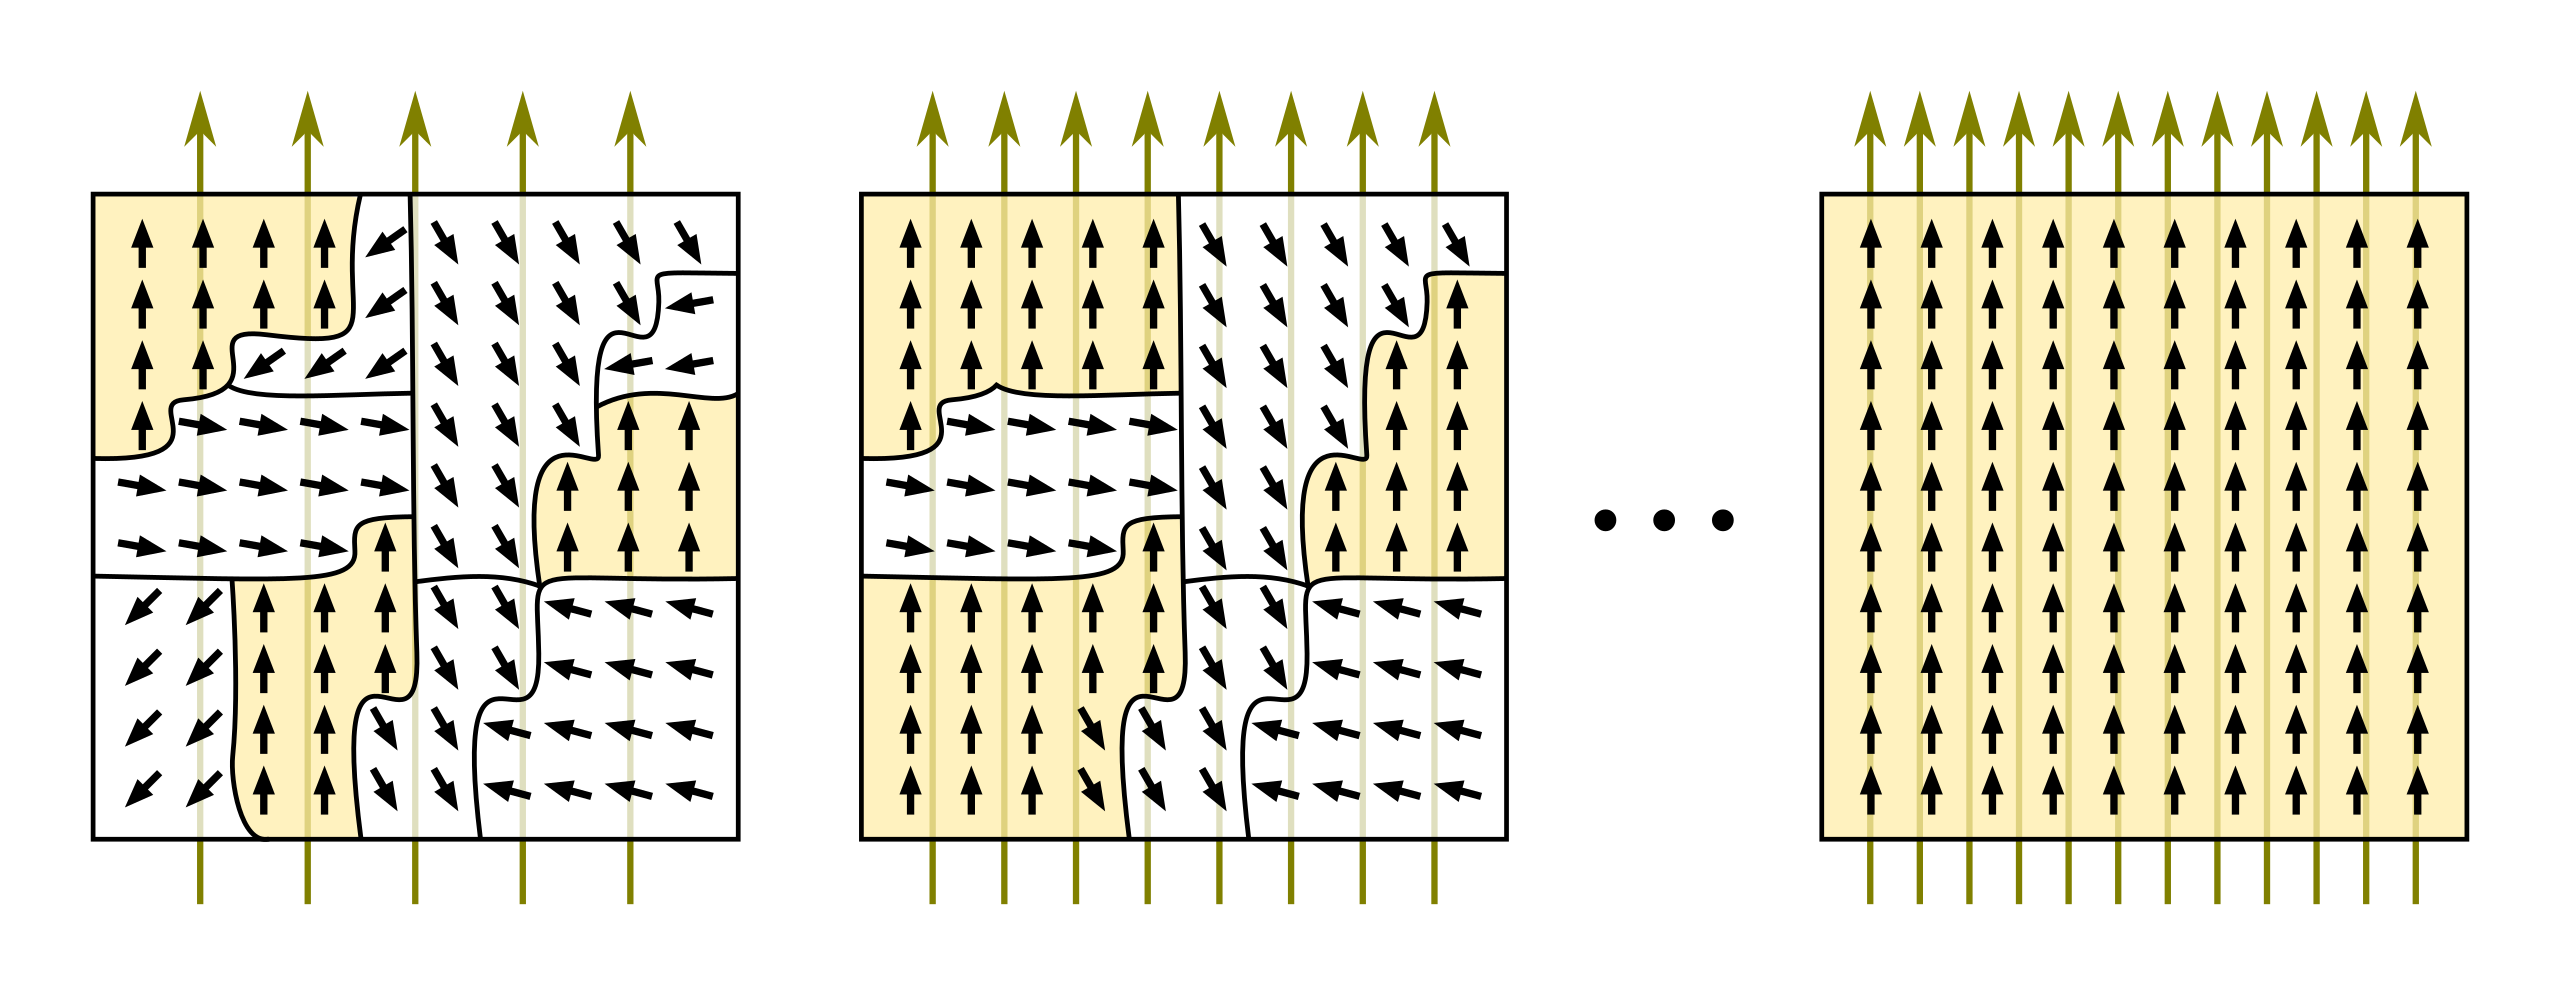
\includegraphics[width=1.0\textwidth]{03_Ressourcen/Bilder/growing-magnetic-domains.svg.png}
    \caption{Schematische Darstellung der Domänenentwicklung bei Anlegen eines äußeren Magnetfeldes, nach \cite{image-Growing_magnetic_domains-MikeRun}}
    \label{fig:weiss_bezirke}
\end{figure}

Infolge einer steigenden Feldstärke \gls{sym:H} vergrößern sich energetisch günstig orientierte Domänen. Dieser Prozess wird initial maßgeblich durch die Verschiebung der Bloch-Wände getrieben. Bei einer weiteren Erhöhung der Feldstärke setzt die Drehung der magnetischen Momente innerhalb der Domänen ein, bis eine vollständige Ausrichtung in Feldrichtung erreicht ist. Dieser Endzustand definiert die magnetische Sättigung. In diesem Bereich führt eine weitere Steigerung der Feldstärke \gls{sym:H} nur noch zu einer marginalen Zunahme der Flussdichte \gls{sym:B}, da die maximale Magnetisierung des Materials nahezu erreicht ist~\cite[Kap.~11]{book-Magnetisches_Feld_Moeller-Harriehausen}.

Diese nichtlineare Domänenumordnung bewirkt, dass die effektive Permeabilität \gls{sym:mur} im Sättigungsbereich drastisch sinkt. Für Messstromwandler resultiert daraus eine reduzierte Messgenauigkeit bei hohen Primärströmen \gls{sym:I_p} oder bei überlagerten magnetischen Fremdfeldern~\cite[Kap.~11]{book-Magnetisches_Feld_Moeller-Harriehausen}\cite[S.~73]{book-Technologie_Messwandler-Minkner}.

Zusätzlich zur Nichtlinearität tritt das Phänomen der Hysterese auf. Dies beschreibt den Umstand, dass die Flussdichte \gls{sym:B} bei veränderlicher Feldstärke \gls{sym:H} nicht nur vom aktuellen Wert, sondern vom vorherigen Magnetisierungszustand abhängt. Abbildung~\ref{fig:bh-hysterese} verdeutlicht dieses Verhalten im $B$-$H$-Diagramm~\cite[Kap.~11]{book-Magnetisches_Feld_Moeller-Harriehausen}.

Die Neukurve beschreibt den initialen Magnetisierungsvorgang eines unmagnetisierten Materials bis zur Sättigung. Bei anschließender Reduktion der Feldstärke \gls{sym:H} verläuft die Flussdichte \gls{sym:B} entlang einer Hystereseschleife und kehrt nicht zum Nullpunkt zurück. Ursächlich hierfür sind irreversible Verschiebungen der Bloch-Wände, die durch Gitterdefekte im Kristallgefüge behindert werden. Bei einer Feldstärke von \gls{sym:H} = \num{0} verbleibt die Remanenzflussdichte \gls{sym:Br}. Zur vollständigen Entmagnetisierung muss eine Gegenfeldstärke aufgebracht werden, deren Betrag als Koerzitivfeldstärke \gls{sym:Hc} definiert ist~\cite[Kap.~11]{book-Magnetisches_Feld_Moeller-Harriehausen}.

\begin{figure}[H]
    \centering
    \includegraphics[width=1.0\textwidth]{03_Ressourcen/simulation/hysterese/hysterese_kurve_final_colors.pdf}
    \caption{Schematische Darstellung von Neukurve und Hystereseschleife im $B$-$H$-Diagramm}
    \label{fig:bh-hysterese}
\end{figure}

Die von der Hystereseschleife umschlossene Fläche korreliert direkt mit den magnetischen Ummagnetisierungsverlusten pro Zyklus. In der Messtechnik werden daher bevorzugt weichmagnetische Werkstoffe mit geringer Koerzitivfeldstärke \gls{sym:Hc} und schmaler Hystereseschleife eingesetzt, um die Remanenz \gls{sym:Br} sowie die Verlustleistung zu minimieren~\cite[Kap.~11.12.1]{book-Magnetisches_Feld_Moeller-Harriehausen}\cite{book-Magnetisches_Feld_Moeller-Harriehausen, website-Magnetisierungskurve-Mietke}.



\subsubsection{Störeinflüsse bei Messstromwandlern}
\label{sec:stoerfelder_schaltanlagen}

Die Messgenauigkeit von Stromwandlern im Betrieb wird maßgeblich von externen und systembedingten Faktoren beeinflusst. Die wesentlichen Störeinflüsse gliedern sich in die drei Kategorien der fehlerhaften Bürdenbeschaltung, der Einwirkung externer magnetischer Fremdfelder sowie der geometrischen Positionierung des Primärleiters~\cite[S.~65]{book-Technologie_Messwandler-Minkner}.

\paragraph{Einfluss der Bürde}
\label{par:einfluss_buerde}

Die Impedanz der Bürde determiniert das Betriebsverhalten des Stromwandlers maßgeblich. Wie im vereinfachten Ersatzschaltbild (Abbildung~\ref{esb:wandler_vereinfacht}) dargestellt, setzt sich der Sekundärkreis aus der Innenimpedanz der Wicklung und der externen Bürde zusammen. Eine Vergrößerung des Gesamtimpedanzbetrags im Sekundärkreis erfordert eine höhere induzierte Spannung \gls{sym:Uo} zur Aufrechterhaltung des eingeprägten Sekundärstroms \gls{sym:I_sec}~\cite[S.~65--67]{book-Technologie_Messwandler-Minkner}.

Unter Berücksichtigung der Streuinduktivität der Sekundärwicklung \(L_s\) sowie einer induktiven Bürde \(L_B\) werden die Wicklung und die Bürde durch die komplexen Zeigerimpedanzen
\begin{equation}
    \underline{Z}_s = R_s + \mathrm{j}\,\omega L_s,
    \qquad
    \underline{Z}_B = R_B + \mathrm{j}\,\omega L_B,
    \qquad \omega = 2\pi f
    \label{eq:impedanzen}
\end{equation}
beschrieben. Da beide Impedanzen im Sekundärkreis in Serie liegen, ergibt sich für die induzierte Spannung
\begin{equation}
    \underline{U}_o = \underline{I}_s \cdot (\underline{Z}_s + \underline{Z}_B)
    = \underline{I}_s \cdot \bigl((R_s+R_B) + \mathrm{j}\,\omega(L_s+L_B)\bigr).
    \label{eq:spannung_impedanz_zeiger}
\end{equation}
Für den Effektivwert folgt daraus die Beziehung
\begin{equation}
    U_o = I_s \cdot \left|\underline{Z}_s + \underline{Z}_B\right|
    = I_s \cdot \sqrt{(R_s+R_B)^2 + \bigl(\omega(L_s+L_B)\bigr)^2}.
    \label{eq:spannung_impedanz}
\end{equation}

Gemäß der Hauptgleichung des Transformators besteht ein proportionaler Zusammenhang zwischen der induzierten Spannung und dem magnetischen Fluss \gls{sym:Phi} im Kern~\cite[S.~67]{book-Technologie_Messwandler-Minkner}:

\begin{equation}
    U_o = 4{,}44 \cdot f \cdot N_s \cdot \Phi.
    \label{eq:trafo_hauptgleichung}
\end{equation}

Durch Substitution von Gleichung \eqref{eq:spannung_impedanz} in \eqref{eq:trafo_hauptgleichung} ergibt sich für den Fluss \gls{sym:Phi}:
\begin{equation}
    \Phi
    = \frac{I_s \cdot \sqrt{(R_s+R_B)^2 + \bigl(\omega(L_s+L_B)\bigr)^2}}
           {4{,}44 \cdot f \cdot N_s}.
    \label{eq:fluss_buerde_mit_induktivitaet}
\end{equation}

Aus Gleichung \eqref{eq:fluss_buerde_mit_induktivitaet} wird ersichtlich, dass nicht nur ein Anstieg des ohmschen Bürdenanteils \gls{sym:RB}, sondern ebenso eine Zunahme der induktiven Anteile den erforderlichen Spannungsbetrag und damit den magnetischen Fluss \gls{sym:Phi} erhöht. Übersteigt dieser Fluss die Sättigungsgrenze des Kernmaterials, verlässt der Wandler seinen linearen Arbeitsbereich, wodurch die Messabweichung signifikant zunimmt~\cite[S.~67, S.~73]{book-Technologie_Messwandler-Minkner}.

\paragraph{Magnetische Fremdfelder}
\label{sec:theorie_fremdfelder}

Nach dem Durchflutungsgesetz ist jeder stromdurchflossene Leiter von einem konzentrischen Magnetfeld umgeben. Befinden sich mehrere Leiter in unmittelbarer Nähe zueinander, überlagern sich deren magnetische Felder gemäß dem Superpositionsprinzip. Die Abhängigkeit der magnetischen Flussdichte \gls{sym:B} vom Abstand \gls{sym:r} zu einem geraden, unendlich langen Leiter wird durch das Gesetz von Biot-Savart beschrieben~\cite[S.~343]{book-Kuepfmueller_Theo_ETechnik-Mathis}\cite[Kap.~4.5.4]{book-Physik_Ingenieure-Hering}\cite[S.~333]{book-Kuepfmueller_Theo_ETechnik-Mathis}:

\begin{equation}
    B(r) = \frac{\mu_0 \cdot I_p}{2 \pi \cdot r}
    \label{equ:biot_savart}
\end{equation}

Ein Stromwandler ist idealerweise so konstruiert, dass sein Kern ausschließlich den magnetischen Fluss des umschlossenen Primärleiters führt. In der Praxis verlaufen die Sammelschienen in Hochstrom-Schaltanlagen jedoch oft parallel und mit geringem Abstand zueinander. Die von Nachbarleitern emittierten Magnetfelder können als Streufluss in den Eisenkern eindringen und sich dem Nutzfluss überlagern. Zur Quantifizierung dieses Effekts wird ein Berechnungsansatz der MBS AG herangezogen, der die zusätzliche Flussdichte \gls{sym:B_fremd} ermittelt~\cite[S.~75]{book-Technologie_Messwandler-Minkner}\cite{pdf-Accuracy_Current_Transformers-Pfuntner}\cite{website-Fremdfeldkompensierte_Wandler-MBS}:

\begin{equation}
    B_{\text{Fremd}} \approx \num{1,00} \cdot 10^{-6} \cdot I_{p} \cdot \frac{R + \num{0,50} \cdot W}{A} \cdot \log_{10}\left(\frac{D+R}{D-R}\right)
    \label{equ:stray_flux_mbs}
\end{equation}

\begin{figure}[H]
    \centering
    \includegraphics[width=1.0\textwidth]{03_Ressourcen/zeichnungen/aufbau_abschätzung_fremdfeld.drawio.pdf}
    \caption{Geometrische Parameter zur Berechnung des Fremdfeldeinflusses}
    \label{pic:aufbau_abschaetzung_fremdfeld}
\end{figure}

Die Variablen sind definiert als induzierte magnetische Fremdflussdichte \gls{sym:B_fremd} (in \unit{T}), Primärstrom \gls{sym:I_p} (in \unit{A}), äußerer Kernradius \gls{sym:R} (in \unit{m}), Leiterbreite \gls{sym:W} (in \unit{m}), Eisenquerschnitt \gls{sym:A} (in \unit{m^2}) und Außenphasenabstand \gls{sym:D} (in \unit{m}).

\begin{figure}[H]
    \centering
    \includegraphics[width=1.0\textwidth]{03_Ressourcen/simulation/fremdfeld_ra_pfunder/Vergleich_Geometrie_und_Strom.pdf}
    \caption{Einfluss von Kerngröße und Stromstärke auf den zusätzlichen Streufluss}
    \label{pic:sim_streufluss_abhaengigkeit}
\end{figure}

Abbildung~\ref{pic:sim_streufluss_abhaengigkeit} visualisiert den eingekoppelten magnetischen Fremdfluss \gls{sym:Phi_fremd}. Ein Vergleich zwischen einem kleinen (blau) und einem großen Kern (rot) zeigt, dass ein geometrisch größerer Kern aufgrund seiner Ausdehnung absolut gesehen mehr Störfluss aufnimmt. Die höhere Robustheit großer Kerne resultiert jedoch aus der Relation zur Sättigungsgrenze, welche durch die resultierende Flussdichte \gls{sym:B_res} bestimmt wird~\cite[Kap.~11]{book-Magnetisches_Feld_Moeller-Harriehausen}:

\begin{equation}
    B_{\text{res}} = B_{\text{Nutz}} + \underbrace{\frac{\Phi_{\text{Fremd}}}{A}}_{B_{\text{Fremd}}}
    \label{eq:b_phi_relation}
\end{equation}

Ein größerer Kernquerschnitt \gls{sym:A} kompensiert die höhere Flussaufnahme, sodass der Anstieg der Flussdichte gering bleibt. Der absolute Fremdfluss \gls{sym:Phi_fremd} ist dabei unabhängig vom Querschnitt:

\begin{equation}
    \Phi_{\text{Fremd}} \approx \num{1,00} \cdot 10^{-6} \cdot I_{p} \cdot (R + \num{0,50} \cdot W) \cdot \log_{10}\left(\frac{D+R}{D-R}\right)
    \label{eq:phi_fremd_herleitung}
\end{equation}

\paragraph{Exzentrische Positionierung der Kupferschiene}
\label{par:exzentrische_positionierung}

Wie in Abschnitt \ref{sec:kompensationswicklungen} dargelegt, ist eine ideal zentrierte Montage der Kupferschienen in der Praxis oft nicht realisierbar. Bereits geringfügige Abweichungen führen zu einer inhomogenen Flussverteilung im Kern und begünstigen lokale Sättigungseffekte~\cite[S.~76]{book-Technologie_Messwandler-Minkner}.

\begin{figure}[H]
    \centering
    \includegraphics[width=1.0\textwidth]{03_Ressourcen/simulation/wandler_mit_kupferschine/wandler_kupferschine_1p.pdf}
    \caption{Simulierter Verlauf des magnetischen Flusses entlang des mittleren Kernumfangs bei zentrierter und exzentrischer Primärleiterposition}
    \label{pic:sim_exzentrische_montiert}
\end{figure}

Abbildung~\ref{pic:sim_exzentrische_montiert} verdeutlicht den simulierten Verlauf des magnetischen Flusses \gls{sym:Phi} entlang des Kernumfangs. Während die zentrierte Anordnung (blau) eine homogene Verteilung aufweist, führt die exzentrische Position (orange) zu einer Asymmetrie. In leiternahen Bereichen steigt der Fluss \gls{sym:Phi} an, während er auf der gegenüberliegenden Seite abfällt. Sofern die Sekundärwicklung \gls{sym:Ns} nicht vollkommen gleichmäßig verteilt ist, resultieren aus dieser Inhomogenität Messabweichungen~\cite[S.~76]{book-Technologie_Messwandler-Minkner}.

\subsection{Messabweichung und Fehlerfortpflanzung}
\label{sec:messabweichung_fehlerfortpflanzung}

Zur Sicherstellung der normativ geforderten Genauigkeitsklassen wird in der Prüftechnik das Prinzip der Vergleichsmessung angewendet. Hierbei werden der zu prüfende Wandler und ein hochpräzises Referenznormal primärseitig von demselben Primärstrom \gls{sym:I_p} durchflossen. Da die Fehlercharakteristik des Normals bekannt und dessen Eigenabweichung vernachlässigbar klein ist, lässt sich die Messabweichung des Prüflings unmittelbar aus der Differenz der sekundärseitigen Ausgangssignale ableiten~\cite{norm-DIN_EN_61869_2-Messwandler_Teil2-DIN}.

Gemäß der Norm DIN EN 61869-2 sind zwei zentrale Kenngrößen zu ermitteln. Die Übersetzungsmessabweichung \gls{sym:epsilon} beschreibt die prozentuale Differenz der Stromamplituden und wird nach Gleichung \eqref{eq:messabweichung_epsilon} bestimmt:

\begin{equation}
    \varepsilon = \frac{k_n \cdot I_{s} - I_{p}}{I_{p}} \cdot \SI{100,00}{\percent}
    \label{eq:messabweichung_epsilon}
\end{equation}

Hierbei entspricht \gls{sym:kn} dem Bemessungsübersetzungsverhältnis. Die zweite essenzielle Kenngröße ist der Fehlwinkel \gls{sym:deltaphi}, welcher die Phasenverschiebung zwischen dem primären und dem sekundären Stromzeiger definiert. Für die Validierung ist zudem die Belastung mit der Nennbürde entscheidend, da die Impedanz des Sekundärkreises die magnetische Aussteuerung des Kerns und somit die resultierenden Fehlerwerte maßgeblich determiniert~\cite{norm-DIN_EN_61869_2-Messwandler_Teil2-DIN}.
